% $Id$
\documentclass[twocolumn,prd,nofootinbib]{revtex4}


\newcommand\ForInternalReference[1]{}
\newcommand\SkipForEarlyCirculation[1]{}
\newcommand\AddedResponse[1]{{\color{blue} {#1}}}
%\newcommand\SkipForEarlyCirculation[1]{#1}
\newcommand\SkipPP[1]{}
\usepackage{verbatim}
\usepackage{graphicx}
\usepackage{dcolumn}
\usepackage{bm}
\usepackage{color}
\usepackage{xspace}
\usepackage{url}
\usepackage{amsmath}
%\usepackage{adjustbox}
\usepackage{float}
\usepackage{multirow}
\usepackage{amssymb}
%
%
\usepackage{times}
%
%
%
\newcommand\optional[1]{}

%
\newcommand\E[1]{\left\langle #1\right\rangle}
\newcommand\qmstate[1]{\left|#1\right \rangle}
\newcommand\qmstateKet[1]{\left\langle#1\right|}
\newcommand\qmstateproduct[2]{\left\langle#1|#2\right\rangle}
\newcommand\qmoperatorelement[3]{\left\langle#1\left|#2\right|#3\right\rangle}
\newcommand\qmoperator[1]{{\bf #1}}
%
\newcommand\Y[1]{{{}_{#1}Y}}

\newcommand\lnL{ \ln {\cal L}}
\newcommand\lnLmarg{ \ln{\cal L}_{\rm marg}{}}
\newcommand\unit[1]{{\rm #1}}

\newcommand\rapidPEOrig{rapid\_pe1}
\newcommand\ILE{ILE}
\newcommand\editremark[1]{{\color{red} #1}}
%
%
%
\usepackage{color}
\definecolor{amber}{rgb}{1.0, 0.75, 0.0}
\definecolor{orange}{rgb}{1.0, 0.5, 0.0}
\definecolor{amaranth}{rgb}{0.9, 0.17, 0.31}
\def\fixme#1{\textcolor{red}{#1}}
\newcommand{\Richard}[1]{ {\color{blue}{#1}}}
\newcommand{\ros}[1]{ {\color{blue}{#1}}}
%

%

%
%
%
%
\graphicspath{{./figures/}}
\newcommand{\mc}{{\cal M}}
\newcommand{\Ms}{M_{\odot}}
\newcommand\LambdaTilde{\widetilde{\Lambda}}
\newcommand\DeltaLambdaTilde{\delta \widetilde{\Lambda}}
%
\def\ltsima{$\; \buildrel < \over \sim \;$}
\def\simlt{\lower.5ex\hbox{\ltsima}}
\def\gtsima{$\; \buildrel > \over \sim \;$}
\def\simgt{\lower.5ex\hbox{\gtsima}}

\newcommand\prx{Phys.~Rev.~X}
\def\aj{Astronomical Journal}                 %
\def\apj{Astrophysical Journal}                %
\def\apjl{Astrophysical Journal}             %
\def\pasj{PASJ}
\def\apjs{ApJS}              %
\def\mnras{MNRAS}            %
\def\prd{Phys.~Rev.~D}       %
\def\prl{Phys.~Rev.~Lett}    %
\def\cqg{Class.~Quant.~Grav.~}%
\def\araa{ARA\&A}             %
\def\nat{Nature}              %
\def\aap{A\&A}                %
\def\aapr{A\&A~Rev.~}    %
\def\pasp{PASP}    %
\def\sovast{Soviet Ast.}
%
%

\newcommand{\IMRPD}{\textsc{IMRPhenomD}\xspace}
\newcommand{\IMRPDT}{\textsc{IMRPhenomD\_NRTidal}\xspace}
\newcommand{\IMRP}{\textsc{IMRPhenomPv2}\xspace}
\newcommand{\SEOBP}{\textsc{SEOBNRv3}\xspace}
\newcommand{\SEOBA}{\textsc{SEOBNRv4}\xspace}
\newcommand{\SEOBAROM}{\textsc{SEOBNRv4\_ROM}\xspace}
\newcommand{\NRSur}{NRSur7dq2\xspace}
\newcommand{\TEOB}{SEOBNRv4T\xspace}
\newcommand{\Resum}{TEOBResumS\xspace}
\newcommand\RIFT{RIFT}
\newcommand{\Taylor}{TaylorF2\xspace}
\newcommand\PaperDetection{\underline{LVC-detect}\cite{DiscoveryPaper}}
\newcommand\PaperPE{\underline{LVC-PE}\cite{PEPaper}}
\newcommand\PaperTestGR{\underline{LVC-TestGR}\cite{TestingGRPaper}}
\newcommand\PaperPENRMethods{\underline{PE+NR-Methods}\cite{gwastro-PENR-Methods-Lange}}
\newcommand\PaperAstro{\underline{LVC-Astro}\cite{AstroPaper}}
\newcommand\PaperBurst{\underline{LVC-Burst}\cite{BurstPaper}}
\newcommand\PaperRates{\underline{LVC-Rates}\cite{RatesPaper}}
\newcommand\PaperStochastic{\underline{LVC-Stochastic}}
\newcommand\PaperSEOBNRvthree{\underline{LVC-SEOBNRv3}\cite{SEOBv3Paper}}

\def\RIT{Center for Computational Relativity and Gravitation, Rochester Institute of Technology, Rochester, New York 14623, USA}

\begin{document}
\renewcommand{\arraystretch}{1.5}
\title{Population Inference of Non-Spinning Eccentric Binary Black Holes}
%\author{R. O'Shaughnessy}
\affiliation{\RIT}
%\author{M. Zeeshan}

\affiliation{\RIT}
\begin{abstract}
The astrophysical mergers produces gravitational waves which carries the plethora of information of their generator. We use those gravitational waves signals to make the inference of population properties. In this study, we made the inference of non-spinning, eccentric binary black holes. As the current GWs signals do not include the eccentricity in their parameters estimation, we made the four synthetic population with different eccentricity using power law model. We used the MCMC method to constrain the model and successfully recovered the eccentricity from the population.
\end{abstract}
\maketitle

\section{Introduction}
Black holes are intriguing and compact objects in the universe \cite{Frolic_BH_Book_2011}. They get interesting and enlightening when they coalesce and emit gravitational waves (GWs) \cite{Indrajit_GW_intro_1999}. These waves carry insightful information about the BBH system, such as mass, spin, period, eccentricity, distance, location, formation, and evolution. In addition, gravitational waves may be the only way to detect those chaotic mergers in space because there was no physical evidence before LIGO's \cite{LIGO_2015} first detection of a BBH merger. Afterward, LIGO-VIRGO-KAGRA (LVK) \cite{LIGO_2015,VIRGO_2012,virgo-2015,kagra-2013} are detecting  gravitational waves from various compact binaries such as binary black holes (BBHs), binary neutron stars (BNS), and binary made of neutron stars and black holes. The sensitivity of detectors is increasing with time, leading to a higher detection in each observing run, and we will have hundreds of events in future runs \cite{detection_rate_2016,detection_rate_2015}.

Among all the confirmed detection, most of them shows a nearly circular orbit in LVK frequency band. However, we have growing evidences that suggests BBHs such as GW15901 may exhibit unambiguous eccentricity or faint signatures \cite{Gamba_2022_GW190521_dynamical,yumeng-2023,Isobel-2022} which can give us better details about the formation scenario. In addition to have faint signature in LIGO frequnecy band, we may have the higher eccentric mergers at the lower frequency searches \cite{sesana-2016,chen-2017}.
There are various scenarios which may develop eccentricity in BBHs orbits, such as stellar scattering, dynamic interactions in dense environments, or a third object in a binary. The existence of eccentricity makes things difficult to comprehend and challenges the current understanding of the formation, environment, and evolution of such compact objects. We also have the reasonable disagreement on the masses, spin, event rate and formation scenarios \cite{LSC-BBH-2016,LSC-GW150914-2016} which leads to new models \cite{Mandel-2016,marchant-2016}. The increment of discovery rate of GWs is constantly challenging the theoretical models and pushing the researcher to develop more sophisticated models. 

Therefore, identifying and understanding the populations of EBBHs with growing number of detection of compact binaries will give us more insightful information about formation and evolution of massive stars from birth to death over cosmic time. 


Eccentricity is the sharply decreasing function of GWs frequency. \cite{peters-1964}.

The GWs produced by the dynamical formed BBHs can carry the non-negligible eccentricity within the LIGO frequency band \cite{samsing-2018, Rodriguez-2018,Antonini-2014}. 

Currently, LVK is using the ciruclar wave form. However, studies shows that we need to consider the multiple formation channels to get the better understaing because, each channel does not contribute more than 70\% of the observation sample of binary black holes \cite{zevin-2021}.


Till now, no modelled search for eccentric signals due to lack of inspiral-merger-ringdown waveform models with eccentricity.

Unmodelled searches mostly efficient for higher mass system whereas effect of eccentricity will be more in the low mass systems.

Despite this, little is known about the formation channels of these mergers. It is difficult to characterize the formation channel of a given merger from the parameters that are usually measured, mass and spin. Unfortunately, many different formation scenarios can produce these combinations. One possible way of determining how a binary may have formed is to better constrain the dynamics of the merger, in addition to these parameters.

Specifically, orbital eccentricity may help distinguish different populations of compact binaries. Slow-forming, low-energy binaries tend to start with low eccentricities, and gravitational wave radiation further circularizes their orbits \cite{Peters-1964}. However, binaries formed in more violent, energetic environments, such as globular clusters, can have large eccentricities. These binaries are expected to retain measurable eccentricities after entering the LIGO sensitivity band, potentially making orbital eccentricity an important parameter in determining formation channel \cite{Rod-2018,zevin-samsing-2019}.



Recent works investigates how measurements of black hole mass and spin distributions can elucidate the population properties of binary black holes \cite{Dan_2019,Michael-2015,Mandel_2017_Errors,samsing-hamers-2019,belczynski-2016,Colm-2017,Akinobu-2017,Michael-zevin-2017,farr-2017-nature,Richard-2017-natal-kicks,Dan-Richard-2018}. we also have the research to constrain the population models with eccentricity \cite{lower-2018-ecc-pop}. It has also been suggested that the future
Laser Interferometer Space Antenna (LISA) will be able to
observe nearby stellar-mass BBH during the early inspiral
phase. These observations would allow for long-term
tracking of BBH orbital properties which can be used to
infer the formation mechanism \cite{Breivik-2016}.



In Sec. \ref{sec:methods} we described the Bayesian statistical methods which we used to make the population inference, and brief method of volume-time estimation. We also explained the previously constructed\cite{fishbach-2017,2018talbot_bbh_model} power law model with modification for eccentricity by using truncated normal distribution. we used this model to generate synthetic population and it's inference. The Sec. \ref{sec:syn_pop} describes that how we have created synthetic population using power law model and then adding error into each event to make population closer to real population detectable by LVK. Secodnly, we explained about the scaling by removing the eccentricity from the synthetic events to make the comparison between EBBHs and NEBBHs population. 

%In addition to electromagnetic waves spectrum, the gravitational waves also provides the completely new domain to study the formation and environment of such compact object. 





%Eccentricity is the unique signature of strong events and can be measured with GWs.


%Most of the eccentric binary black holes (EBBHs) are driven by low masses $(10M_\odot-30M_\odot)$ and if any component of the binary has mass less than $30 M_\odot$ then only $10\%$ of them are able to maintain eccentricity near the last stable orbit.  \cite{mass_ecc_limit_2018}. Therefore,  in this study, we  will consider binaries with non-spinning $(\chi_i = 0)$, eccentric $(0-0.5)$ and moderate mass range $(10M_\odot-50M_\odot)$. In addition, we will use mass ratio $q=m_1/m_2$ with condition $m_1>m_2$ and total mass $M=m_1+m_2=100M_\odot$.



\section{Methods}
\label{sec:methods}

The coalescing BBH can be completely described by three intrinsic and seven extrinsic parameters. The intrinsic parameters, such as the mass of the binary component ($m_i$), spin $( \chi_i)$, and eccentricity $\epsilon$  are subject to the orbital evolution of the binary. The extrinsic parameters are orientation (orbital phase, polarization, and inclination), sky location (right ascension and declination), luminosity distance, and coalescence time depend on the observer.



\subsection{Hierarchical Bayesian Modeling (HBM)}


We use HBM to constrain the population models with gravitational wave signals. It is also a good choice to consider the sensitivity of LIGO-VIRGO-KAGRA (LVK) and uncertainty in each detection.

In HBM, we have the N number of discrete detections. Those detections provide merger data denoted as $d_1,d_2,d_3,...,d_N$ where each $d_i$ shows a BBH merger. Each $d_i$ has mass, spin, and eccentricity properties. These properties, often called parameters, are denoted by $\lambda_1,\lambda_2,\lambda_3,...,\lambda_i$. Each parameter has its uncertainty, and we express it by the probability of the data given the parameter value. We also refer to it as the likelihood function $\mathcal{L}(\lambda)=p(d|\lambda)$ of one event. A given value of $\lambda$ is obtained from a mathematical model commonly known as a waveform to calculate a likelihood. Once you have a likelihood function, you may use a uniform prior or any other prior to find a posterior probability using the Bayes theorem as given in Eq. \ref{eq:Bayes_ind}

\begin{equation}
\label{eq:Bayes_ind}    
p(\lambda|d) \propto p(d|\lambda) p(\lambda).
\end{equation}

This posterior probability will constrain the properties of each binary, such as mass, spin, and eccentricity. We may infer those parameters using rapid parameter inference on gravitational wave sources via iterative fitting (RIFT): an open source code for parameter estimation (PE) of the binary sources \cite{rift_2018}.



%\begin{itemize}
%    \item We have N discrete detection.
%    \item each detection has data $d_1,d_2,d_3,...,d_N$
%    \item each data point $d_N$ has properties denoted by $\lambda_1,\lambda_2,...,\lambda_i$
%    \item  $ \lambda_i$ are parameters such as mass, spin, eccentricity, and location.
%    \item Each parameter has its uncertainty.
%    \item This uncertainty is described by the probability of the data given the parameter value. We call it the likelihood function of one single event. $\mathcal{L}(\lambda) = p(d|\lambda)$
%    \item the waveform gives the parameter value.
%    \item waveform is a mathematical function.
%    \item Once you have a likelihood function, you can use prior( usually it's uniform: which gives equal probability to each event) to find the posterior. $p(\lambda|d) \propto p(d|\lambda) p(\lambda)$  
    
%\end{itemize}


\subsection{Population Inference}

Now having the PE of individual sources, we will follow the Bayesian framework for population inference. The likelihood of a population parameter $\Lambda$, also considered as uncertainty in $\Lambda$ is equivalent to the probability of the individual sources given the population parameter $\Lambda$ is written as follows. 

\begin{equation}
\label{eq:likelihood_pop}    
\mathcal{L}(\Lambda)\equiv p(d_1,d_2,d_3,...,d_N|\Lambda)
\end{equation}

 

We will use the likelihood given in Eq. \ref{eq:likelihood_pop} in the Bayes theorem given in Eq. \ref{eq:Bayes} to find the posterior probability.

\begin{equation}
\label{eq:Bayes}    
p(\Lambda|d_1,d_2,...,d_N)= \frac{p(\Lambda)p(d_1,d_2,...,d_N|\Lambda)}{p(d_1,d_2,...,d_N)},
\end{equation}
%
where $p(\Lambda|d_1,d_2,d_3,...,d_N)$ is posterior, $p(\Lambda)$ is prior, $p(d_1,d_2,d_3,...,d_N)$ is normalization constant or also known as evidence.

To conduct our analysis for mass and eccentricity distribution, we will use the inhomogeneous Poisson process scaled by rate $\mathcal{R} = \frac{dN}{dtdV_c}$ and parameterize by $\Lambda$ to find the likelihood  $\mathcal{L}(\mathcal{R},\Lambda)\equiv p(D|\mathcal{R},\Lambda)$ of an astrophysical population given the merger rate and parameter $\Lambda$. 

\begin{equation}
\label{eq: likelihood}
\mathcal{L}(\mathcal{R},\Lambda) \propto e^{-\mu(\mathcal{R},\Lambda)}\prod_{n=1}^N\int d\lambda \ell_n(\lambda) \mathcal{R} p(\lambda|\Lambda),
\end{equation}
%
where $\mu(\mathcal{R},\Lambda)$ is the expected number of detection under the given population parametrization $\Lambda$ with the overall rate $\mathcal{R}$. $\ell_n(\lambda)=p(d_n|\lambda)$ is the likelihood of the data $d_n$ given binary parameter.
Finally, we will get our posterior as $p(\mathcal{R},\Lambda | D)\propto p(\mathcal{R},\Lambda)  \mathcal{L}(\mathcal{R},\Lambda)$ by choosing a prior $p(\mathcal{R},\Lambda)$.

These calculations are analytically intractable and must be performed numerically. Specifically, we will use Goodman and Weare's affine invariant Markov chain Monte Carlo (MCMC) \cite{mcmc_paper} to find the posterior distribution of population parameters. This method draws samples from the targeted distribution for $\Lambda$, in our case, it's the power law model given in Eq. \ref{eq:plawg}, then compares it with the given data (collection of individual events) and stores the best-fit sample. We may iterate this as we need and store multiple sample values untill they converge. 
The specific implementation we use is a Python package called EMCEE \cite{emcee_paper}.


\subsection{Volume Time (VT) Estimation}

To make our study realistic, we include the sensitivity of the LVK instruments. This sensitivity is defined by time-volume to which a census of gravitational wave events is sensitive: inferring the product $VT$.  In this expression, $V$ is the characteristic volume with units $Gpc^{3}$, which refers to the possible detection region in the sky for the LVK \cite{Volume_1993}, and $T$ is the time duration of making observations at this sensitivity.  In practice, $VT$ reflects a suitable time-averaged or cumulative sensitivity, as the true network and sensitivity varies over time.
Existing LVK instruments' sensitivity depends primarily on the mass and to a lesser extent on binary spin and (if present) modest eccentricity.  Since we neglect spin in this work, we assume the network will have the same  VT versus mass as was previously estimated  \cite{Dan_2019} for non-spinning, non-eccentric, and no-precessing binaries. Hence, we briefly explain the calculations, see \cite{Dan_2019} for details.

The Eq. \ref{eq:volume} calculates the orientation averaged sensitive volume \cite{Abbott_2016,richard2010volume}

\begin{equation}
\label{eq:volume}
V(\lambda) = \int P((<D(z))/D_n(\lambda))\frac{dV_c}{dz}\frac{dz}{1+z}
\end{equation}    
where $D(z)$ is the luminosity distance for redshift $z$, $V_c$ is the comoving volume. Finally, to compute the average number of detection, we will use Eq. \ref{eq:mu} and keep in mind that the merger will be accepted only if the signal-to-noise ratio exceeds 8 \cite{SNR_2010}.

\begin{equation}
\label{eq:mu}
  \mu(\mathcal{R},\Lambda) = \int(VT)\lambda \mathcal{R}p(\lambda|\Lambda)d\lambda ,
\end{equation}
where $p(\lambda|\Lambda)$ is the probability density function for a random binary in the universe to have intrinsic parameter $\lambda$. Keep in mind that $\lambda$ is equal to all intrinsic and extrinsic parameters.


\subsection{Power law Model}
There are various weak and pure phenomenological population models proposed in previous studies \cite{2016PRXAbbot_BBH_model,2017FishBach_BBH_model,2018talbot_bbh_model}. However, our analysis used the pure truncated power law defined in \cite{2016PRXAbbot_BBH_model,2017FishBach_BBH_model} and Gaussian eccentricity. This model computes the intrinsic probability of $m_1$, $m_2$, and $\epsilon$.  
We also assume that non-zero probability density only exists for $m_{min}\leq m_2 \leq m_1 \leq m_{max}$ and for total mass $M_{max}=m_1+m_2 = 200 M_\odot$. The condition of the total mass is only because of the limitations of the detectors towards the higher masses \cite{2016PRXAbbot_BBH_model}. The generalized form of the truncated power-law model with parameters $\Lambda \equiv  (\alpha, \mathcal{R}, k_m, m_{min}, m_{max}, \sigma_\epsilon, M_{max})$ and random variable $m_1$, $m_2$, and $\epsilon$ has the functional form in Eq. \ref{eq:plawg} within provided mass limit.


\begin{align}
\label{eq:plawg}
p(m_1,m_2,\epsilon) = &C(\alpha,k_m,m_{min},m_{max},M_{max},\epsilon)  
\nonumber \\ & \sqrt{\frac{2}{\pi}} \frac{(m_2/m_1)^{k_m} m_1^{-\alpha} e^{-(\epsilon/\sqrt{2}\sigma_\epsilon)^2}}{(m_1-m_{min})\sigma_\epsilon},
\end{align}
%
where $\alpha$ is the power law index, $\mathcal{R}$ is the merger rate, $m_{min}, m_{max}$ are the minimum and maximum masses of the binary components in the population, and $\sigma_e$ is the orbital eccentricity distribution. The Eq. \ref{eq:plawg} represent a truncated power law for primary mass $m_1$ with index $-\alpha$ and conditional power law distribution $p(m_2|m_1)$ for secondary mass $m_2$ using simple power law, and Gaussian distribution for orbital eccentricity $e$. 
For our analysis, we defined a constant of integration equal to $\int_V dm_1 dm_2 d\epsilon p(m_1,m_2,\epsilon) = 1$.  Our detectors are sensitive to high-mass BBHs, particularly $M_{max}\geq 200 M_\odot$. Therefore, we will use $k_m=0$ throughout the studies. As a result, we have our reduced form of the truncated power law in Eq. \ref{eq:plaw}

\begin{align}
\label{eq:plaw}
p(m_1,m_2,\epsilon) = \sqrt{\frac{2}{\pi}} \frac{ m_1^{-\alpha}  e^{-(\epsilon/\sqrt{2}\sigma_\epsilon)^2}}{(m_1-m_{min})\sigma_\epsilon}
\end{align}

\section{Synthetic Population}
\label{sec:syn_pop}
We have created four synthetic populations by choosing the power law parameters $\alpha = -1$, $m_{min} = 10$, $m_{max}=50$. Each population has the same values for $\alpha$, $m_{min}$, and $m_{max}$ except $\sigma_\epsilon$. We selected four values for $\sigma_\epsilon = 0.05, 0.1, 0.15, 0.2$, and  generated synthetic population containing $10000$ sources.

\subsection{Synthetic population with eccentricity}

After generating four populations, we find the probability for each event to be detected by computing the VT of each source. Finally, we did the weighting based on these VTs and randomly picked $N=100$ sources from each population to perform our analysis. Our weighted populations with $\sigma_\epsilon=0.05$ and $\sigma_\epsilon=0.2$ are shown in Fig. \ref{fig:pop3d0.05_0.2}.  The complete description of each EBBHs population is provided in Table \ref{tab:pop_prop}.

\begin{figure*}[]
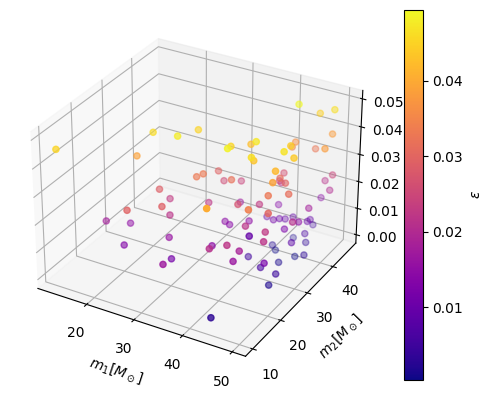
\includegraphics[width=0.45\textwidth]{paper/figures/pop3d_0.05.png}
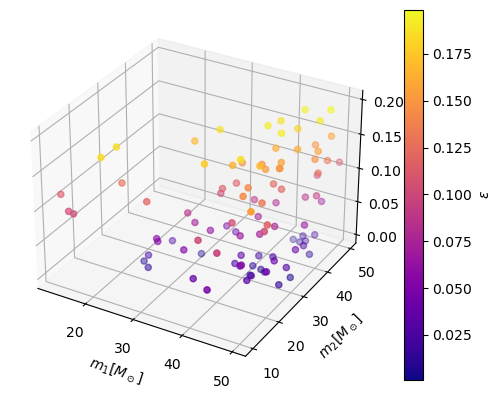
\includegraphics[width=0.45\textwidth]{paper/figures/pop3d_0.2.png}
\caption{\label{fig:pop3d0.05_0.2} Synthetic Population of EBBHs. The left figure represents the population for $\sigma_\epsilon=0.05$ and right figure represents the population for $\sigma_\epsilon=0.2$}
\end{figure*}


\begin{table*}[]
    \centering
    \begin{tabular}{c|cccccc}
        \hline \hline
        Populations & $m_{1_{min}} [M_\odot] $ & $m_{1_{max}} [M_\odot]$ & $m_{2_{min}} [M_\odot]$ & $m_{2_{max}} [M_\odot]$ & $\epsilon_{min}$ & $\epsilon_{max}$\\ \hline
        First  & 12.19 & 49.89 & 10.17 & 46.67 & 0.0004 & 0.0494\\ \hline
        Second  & 15.42 & 49.79 & 10.46 & 47.59 & 0.0003 & 0.0999\\ \hline
        Third  & 16.17 & 49.83 & 10.69 & 47.52 & 0.0002 & 0.148\\ \hline
        Forth  & 12.52 & 49.89 & 10.08 & 49.51 & 0.0012 & 0.1984\\ \hline
    \end{tabular}
    \caption{Population Properties of EBBHs}
    \label{tab:pop_prop}
\end{table*}

To make our study more realistic, we must add the measurement error in each source.  Rather than generate synthetic gravitational wave sources and perform full Bayesian inference, following previous work \cite{Mandel_2017_Errors} we generate mock measurement errors motivated by real parameter inference investigations. The chirp mass and symmetric mass ratio are well-constrained compared to the primary and secondary masses of BBHs. Therefore, we compute them for each event in a population by using the following relations.

\begin{equation}
    M_c^T = \frac{(m_1 m_2)^{3/5}}{(m_1+m_2)^{1/5}},
\end{equation}

\begin{equation}
    \eta^T = \frac{(m_1 m_2)}{(m_1+m_2)^2},
\end{equation}
%
where $M_c^T$ and $\eta^T$ are found using the primary and secondary masses of each event generated by the power law model.
Furthermore, using the following relations, We add the measurement errors in the $M_c^T$ and $\eta^T$.

\begin{equation}
    M_c = M_c^T\left( 1+\alpha (r_0+r ) \frac{12}{\rho}\right),
\end{equation}

\begin{equation}
\eta = \eta^T\left( 1+0.03 (r_0'+r') \frac{12}{\rho}\right),   
\end{equation}
where $r_0$ and $r_0'$ are the random numbers drawn from the standard normal distribution, which will shift the mean of the $M_c$ and $\eta$ distribution with respect to $M_c^T$ and $\eta^T$. The $r$ and $r'$ are the independent and identically distributed arrays of those randomly generated numbers to spread the distribution. The measurement uncertainty is inversely proportional to signal-to-noise ratio $\rho$, drawn from the distribution $p(\rho) \propto \rho^{-4}$, which holds for isotropically distributed sources in a static universe, subject to the threshold $\rho\geq 8$ for detection. The $\alpha =0.1$ is used for the scaling inspired by analyses of mock data with the LALINFERENCE pipeline \cite{alpha_error_2015} and includes the impact of correlation with parameters describing arbitrary remnant spins.

Finally, after adding the measurement errors in the $M_c$ and $\eta$, we will convert them back to $m_1$ and $m_2$ to perform our analysis. We used the following relation for conversion, and it will provide the masses based on the condition $m_1\geq m_2$.

\begin{equation}
    m_1 = \frac{1}{2} M_c \eta^{-3/5} (1+\sqrt{\eta_v}),
\end{equation}

\begin{equation}
    m_2 = \frac{1}{2} M_c \eta^{-3/5} (1-\sqrt{\eta_v}), 
\end{equation}
where $\eta_v = 1-4\eta$, we kept the samples with non-negative values and ignored the negative samples to avoid the square root issues. 

We also added the absolute error in the eccentricity by using the truncated normal distribution scaling at $0.05$ to keep the eccentricity positive.
\textbf{this is important - refer to other papers.  THIS IS REASONABLE FOR LOW MASS BUT VERY OPTIMISTIC FOR HIGH MASS}
STRETCH GOAL: what if you ran again, but with large error?








\subsection{Synthetic population without eccentricity}

To compare the synthetic EBBHs population with the non-eccentric BBHs (NEBBHS), we estimate how our sources would be characterized by parameter inferences which omitted the effects of eccentricity.  Following \cite{2021_scaling_paper}, the following effective chirp mass is well-constrained by observations dominated by the inspiral of a slightly eccentric binary:
\begin{align}
\label{eq:scaling}
M^{ecc} = \frac{M}{(1-\frac{157}{24}\epsilon^2)^{3/5}}
\end{align}
%
Our ansatz for source identification and characterization is that the best-fitting parameters and posteriors are directly related to the true posteriors, except that the recovered chirp mass is given by  Eq. \ref{eq:scaling}.  This process removes the eccentric component from the population only by scaling the masses and omitting the eccentricity. 





%\begin{table*}[]
%    \centering
%    \begin{tabular}{c|cccc}
%        \hline \hline
%        Populations & $m_{1_{min}} [M_\odot] $ & $m_{1_{max}} [M_\odot]$ & $m_{2_{min}} [M_\odot]$ & $m_{_2{max}} [M_\odot]$ \\ \hline
%        First & 12.09 & 49.6 & 10.17 & 46.27 \\ \hline
%        Second & 15.26 & 49.77 & 10.3 & 47.56 \\ \hline
%        Third & 15.96 & 49.5 & 10.62 & 46.60  \\ \hline
%        Forth & 11.86 & 49.76 & 9.67 & 46.99  \\ \hline
%    \end{tabular}
%    \caption{Population Properties of NEBBHs}
    \label{tab:popscl_prop}
%\end{table*}
 

\begin{figure*}

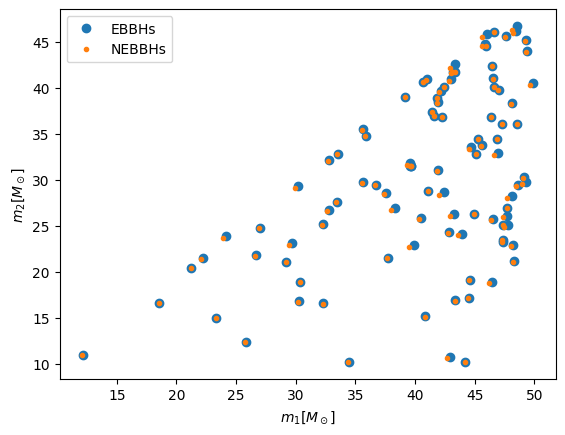
\includegraphics[width=0.45\textwidth]{paper/figures/pop2d_0.05.png}
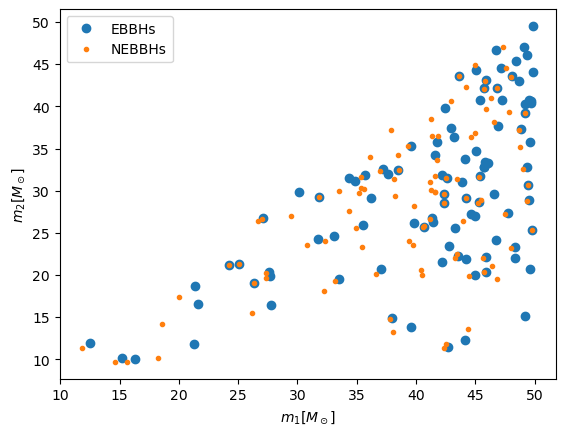
\includegraphics[width=0.45\textwidth]{paper/figures/pop2d_0.2.png}
\caption{\label{fig:pop2d_0.05_0.2} The left figure shows the primary mass vs secondary mass of the EBBHs and NEBBHs with $\sigma_\epsilon =0.05$. The right figure shows the same plot but for $\sigma_\epsilon=0.2$} 

\end{figure*}




%To get the non-eccentric population, we apply the Eq. \ref{eq:scaling} on the population given in the table. \ref{tab:pop_prop}. After applying the scaling equation, we get the new populations with scaled masses, giving us the new minimum and maximum values for the primary and secondary masses given in table \ref{tab:popscl_prop}.
   


The significant effect after scaling is the mass shift, which can be observed in Fig. \ref{fig:pop2d_0.05_0.2}. In this figure, the left-hand side shows the mass shift of the first population generated with smaller $\sigma_\epsilon =0.05$, which leads to a lesser mass shift. However, on the right hand of Fig. \ref{fig:pop2d_0.05_0.2}, one can see the significant mass shift after removing the eccentric component.  This also reflects that we may miss the various sources by ignoring the effect of eccentricity and we notice that sources start missing, which has eccentricity $\epsilon>0.38$.


                            

\section{Population Inference}
\label{sec:pop_inference}
%\renewcommand{\arraystretch}{2}
\begin{table*}[]
    \centering
    \begin{tabular}{c|ccccc}
        \hline \hline
       Inference & $log_{10}(\frac{\mathcal{R}}{Gpc^{-3}yr^-1})$ & $\alpha$ & $m_{min} [M_\odot] $ & $m_{max} [M_\odot]$ & $\sigma_\epsilon$ \\ \hline
      First& $1.42^{+0.58}_{-2.64}$ & $-0.88^{+3.17}_{-1.89}$ & $8.36^{+7.49}_{-3.51}$ & $58.44^{+10.21}_{-24.31}$ & $0.30^{+0.54}_{-0.25}$ \\ \hline
      Second & $1.36^{+0.63}_{-2.65}$ & $-0.93^{+3.29}_{-1.92}$ & $8.71^{+7.36}_{-3.81}$ & $57.84^{+10.81}_{-25.53}$ & $0.33^{+0.51}_{-0.25}$ \\ \hline
      Third & $1.39^{+0.58}_{-2.69}$ & $-0.69^{+2.98}_{-1.95}$ & $9.21^{+6.31}_{-3.99}$ & $57.85^{+10.73}_{-27.04}$ & $0.33^{+0.51}_{-0.23}$  \\ \hline
      Forth & $1.27^{+0.72}_{-2.68}$ & $-0.90^{+3.30}_{-1.98}$ & $8.63^{+7.85}_{-3.72}$ & $57.76^{+11.03}_{-25.82}$ & $0.37^{+0.47}_{-0.23}$  \\ \hline
    \end{tabular}
    \caption{Population Inference for EBBHs}
    \label{tab:inference_EBBHS}
\end{table*}


\begin{table*}[]
    \centering
    \begin{tabular}{c|cccc}
        \hline \hline
        Inference & $log_{10}(\frac{\mathcal{R}}{Gpc^{-3}yr^-1})$ & $\alpha$ & $m_{min} [M_\odot] $ & $m_{max} [M_\odot]$ \\ \hline
      First & $1.85^{+0.14}_{-1.23}$ & $-1.37^{+1.43}_{-0.94}$ & $7.54^{+3.68}_{-3.04}$ & $63.29^{+8.00}_{-13.08}$  \\ \hline
      Second & $1.83^{+0.14}_{-1.38}$ & $-1.12^{+1.47}_{-0.91}$ & $7.69^{+3.88}_{-3.15}$ & $61.91^{+8.59}_{-13.87}$  \\ \hline
      Third & $1.84^{+0.15}_{-1.55}$ & $-0.38^{+1.03}_{-0.96}$ & $8.07^{+3.44}_{-3.27}$ & $61.70^{+8.49}_{-24.26}$   \\ \hline
      Forth & $1.86^{+0.16}_{-1.85}$ & $-0.31^{+1.17}_{-1.14}$ & $6.99^{+8.77}_{-2.58}$ & $61.15^{+8.72}_{-16.84}$  \\ \hline
    \end{tabular}
    \caption{Population Inference for NEBBHs}
    \label{tab:inference_NEBBHS}
\end{table*}


Figure A shows the results of population inference under the most conservative case with $\sigma_\epsilon=0.05$.  In this figure, the ZZ color shows the results of QQ.
%
Most notably, this figure shows that even in the limit of extremely small ecctricity, the impact of eccentricity can be measured from a large population of observations, comparable to the current size.  This result depends of course on our assumption that all binaries are equally likely to have eccentricity, and that our measurement uncertainty in eccentricity is both indpeendent of mass and fairly small, both optimisitic assumptions.  In fact, the overall uncertainty in $\sigma_\epsilon$ is expected: given 100 events, each with a measurement error of $0.05$, we expect $\sigma_\epsilon$ to be measured to of order $0.05/\sqrt{N}$ (handwavy -- really a chisquared distribution,etc).
SUSPECT THAT IF YOU MAKE THIS JUST 3X bigger, STILL GET RESULT -- you will almost always get this result

Also noteworthy is the impact of neglecting eccentricity.  If eccentricity is neglected, then the population inference is biased away from true values: the black contours in the first column do not include the true values for $m_{max}, m_{min}$ example.



Figure B shows the results of population inference under the most optimistic case with $\sigma_\epsilon=0.2$.  In this figure, the ZZ color shows the results of QQ.


we can discuss the corner plots here.

TAKEAWAYS

* Eccentricity can be measured

* If not measured, biases




\begin{figure*}

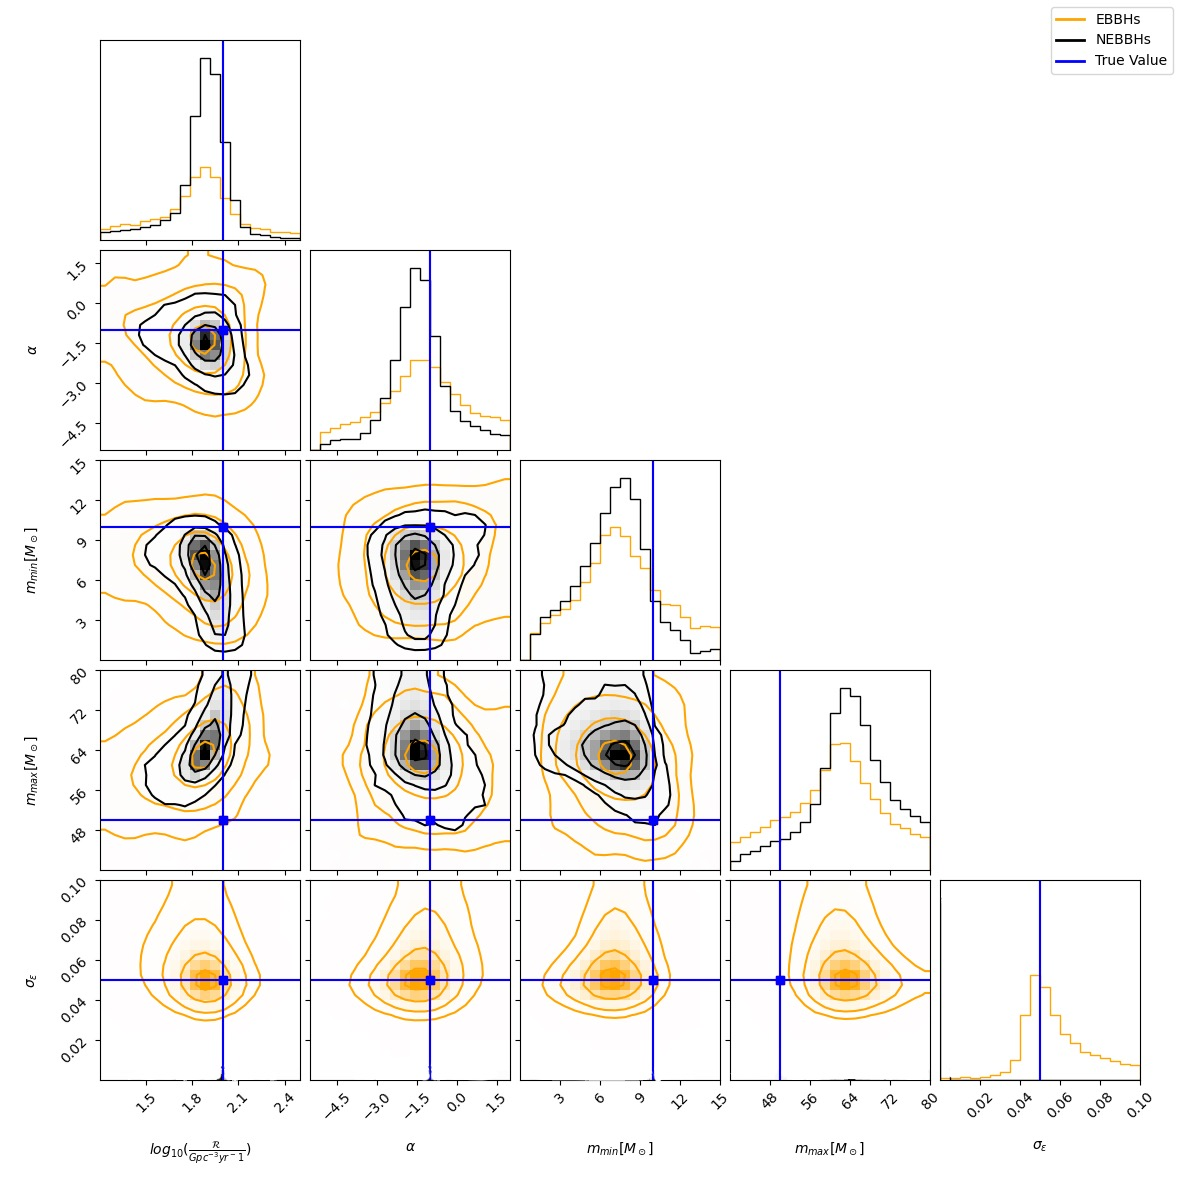
\includegraphics[width=0.95\textwidth]{paper/figures/cor_0.05.png}
\caption{\label{fig:pop3d05}\textbf{Corner Plots for EBBHs and BBHS for $\sigma_\epsilon=0.05$}}

\end{figure*}
Same population.
\begin{figure*}

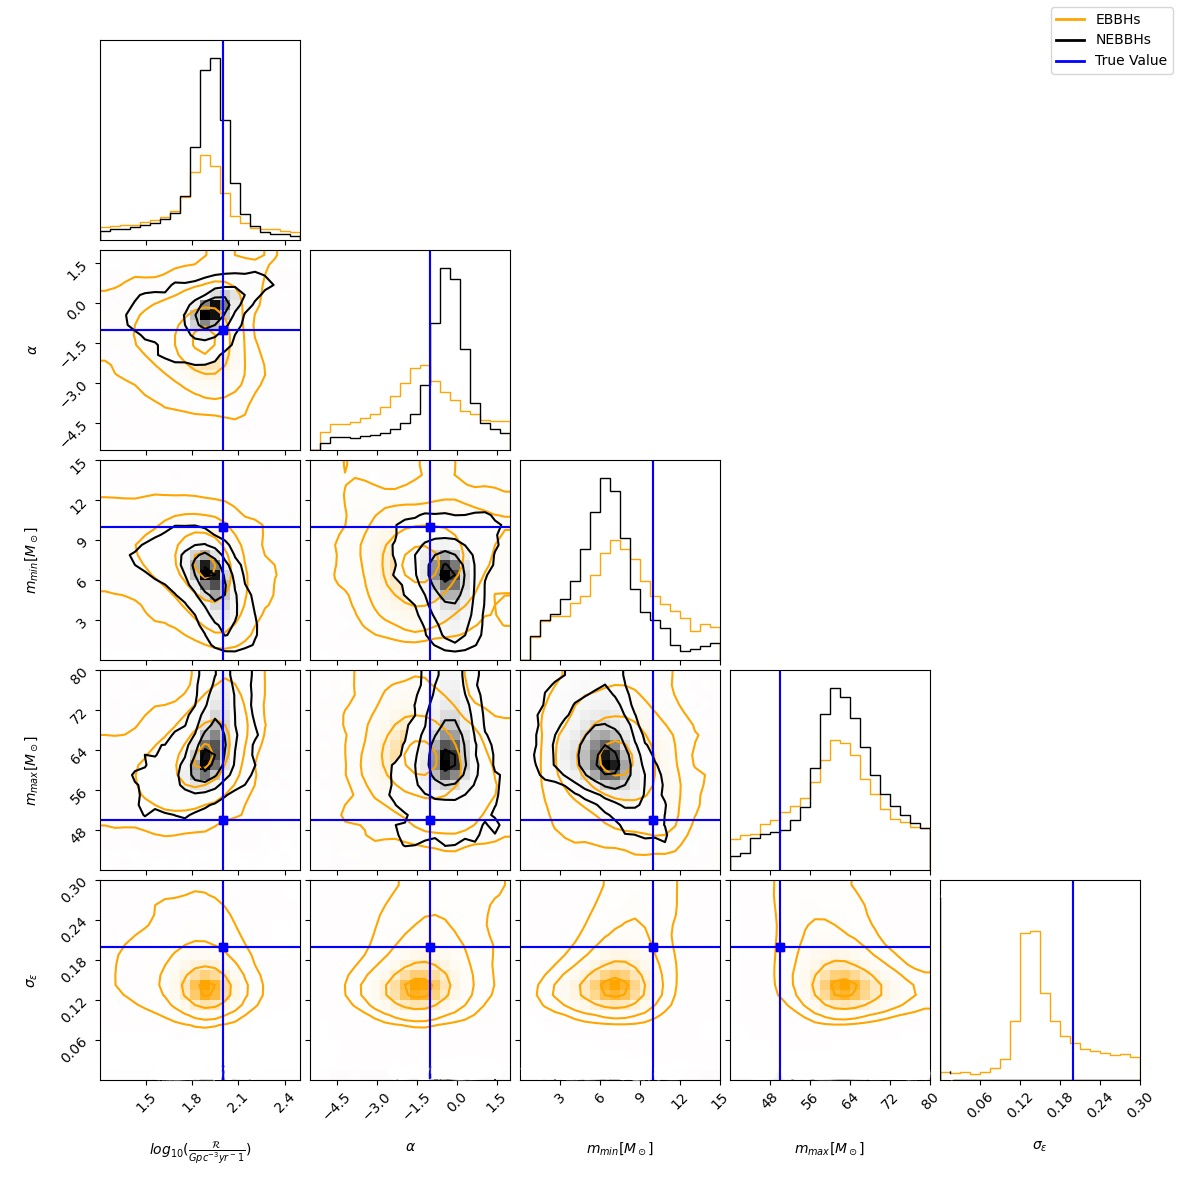
\includegraphics[width=0.95\textwidth]{paper/figures/cor_0.2.png}
\caption{\label{fig:pop3d05}\textbf{Corner Plots for EBBHs and BBHs for $\sigma_\epsilon=0.2$}}

\end{figure*}

Need to write it later. 







% \begin{align} \label{eq:strain_mode}
% h(t,\vartheta,\phi;\bm{\lambda}) = 
% \sum_{\ell=2}^{\infty} \sum_{m=-\ell}^{\ell} \frac{D_{\rm ref}}{D} h^{\ell m}(t;\bm{\lambda}) \Y{-2}_{\ell m} \left(\vartheta, \phi \right) \, ,
% \end{align}


% \begin{widetext}
% \begin{align}
% \ln {\cal L}(\bm{\lambda}, \theta) 
% &= (D_{\rm ref}/D) \text{Re} \sum_k \sum_{\ell m}(F_k \Y{-2}_{\ell m})^* Q_{k,lm}(\bm{\lambda},t_k)\nonumber \\
% &   -\frac{(D_{\rm ref}/D)^2}{4}\sum_k \sum_{\ell m \ell' m'}
% \left[
% {
% |F_k|^2 [\Y{-2}_{\ell m}]^*\Y{-2}_{\ell'm'} U_{k,\ell m,\ell' m'}(\bm{\lambda})
% }
% % \right. \nonumber \\ & \left.
%  {
% +  \text{Re} \left( F_k^2 \Y{-2}_{\ell m} \Y{-2}_{\ell'm'} V_{k,\ell m,\ell'm'} \right)
% }
% \right]
% \label{eq:def:lnL:Decomposed}
% \end{align}
% \end{widetext}

% \begin{eqnarray}
% {\cal L}_{\rm margT} \equiv  \int {\cal L} \frac{dt}{T}
% \label{eq:lnL:tmarg}
% \end{eqnarray}












% \begin{table*}
% \begin{tabular}{lrr|ccccc|rr}
% Version & srate & modes & $\tau_{start}$ & $\tau_{setup}$ & $\tau_{ad}$ & $\tau_{it,like}$ &$\tau_{it,rest}$ &
% $\frac{T_{ILE}}{N_{eval}}$ & GPU \\  %\hline 
%   &   Hz & m & sec & sec & & $\mu$sec & $\mu$sec  &sec  & use  \%\\ \hline 
% % ~/parse_report.sh profile_nogpu_pcdev13.log | more
% CPU & 16384 & $\pm 2 $ & 20 & 2.4 &&540 & 20 &  690  \\ 
%        & 4096 & $\pm 2 $ &   20  &&&& 20 \\ \hline
% % ./parse_report.sh 20190130-profile_nogpu_HM_pcdev13.log  | more
% % /parse_report.sh ./profile_nogpu_HM_lowres_pcdev13.log 
% %    setup time: PrecomputeLikelihoodTerms, includes waveform generation. 
% %   evaluation: FactoredLogLikelihodTimeMarginalized Divide by actual number of calls, since not a block!
% %    
% CPU & 16384 & $\pm 2,\pm 1 $ & 20 & 1.5 && 680 & 20 &  1060  \\ 
%        & 4096 & $ \pm 2, \pm 1 $ &   20 &&&& 20  \\ \hline

%GPU (a) & 16384 & $\pm 2 $  & 20  & & && & 270 \\
%            & 4096 &$\pm 2 $  &  20 &  & & & & 45 \\ \hline

%GPU (b) & 16384 & $\pm 2$ & 20  & 1.8 & 1 & 0.85& 20 &28 & 15\\
%        & 4096 & $\pm 2$  & 20 & $1.2 $ &  1  & 0.75 & 20  & 25\\ \hline

% GPU (b) & 16384 & $\pm 2, \pm 1$ & 20 & 1 && 4.2 & 20  & 38  \\
%        & 4096 & $\pm 2, \pm 1$ & 20 & 1&& 2.5  & 20 & 35 & \\ \hline

% GPU (c) & 16384 & $\pm 2 $  & 20  &6  & & 18&  58&160 &  \\
%             & 4096 &$\pm 2 $  &  20 & 3.7 & & 11  & 58  & 140 & $\simeq 50$ \\
% \end{tabular}
% Compute node at LIGO-WA
% \caption{\label{tab:CostBreakdown}\textbf{Profiling performance: Binary black holes}: Evaluation costs for the
%   marginalized likelihood on default
%   hardware, for a two-mode system $(l,m)=\pm 2$ analyzing $T=8\unit{s}$ of data with a massive binary black hole
%   $m_1=35 M_\odot,M_2=30 M_\odot$.  The last column indicates peak GPU utilization.
% }
%\end{table*}










% \subsection{Binary black hole analysis}
% \label{sec:sub:BBHFull}

% \begin{figure*}

% 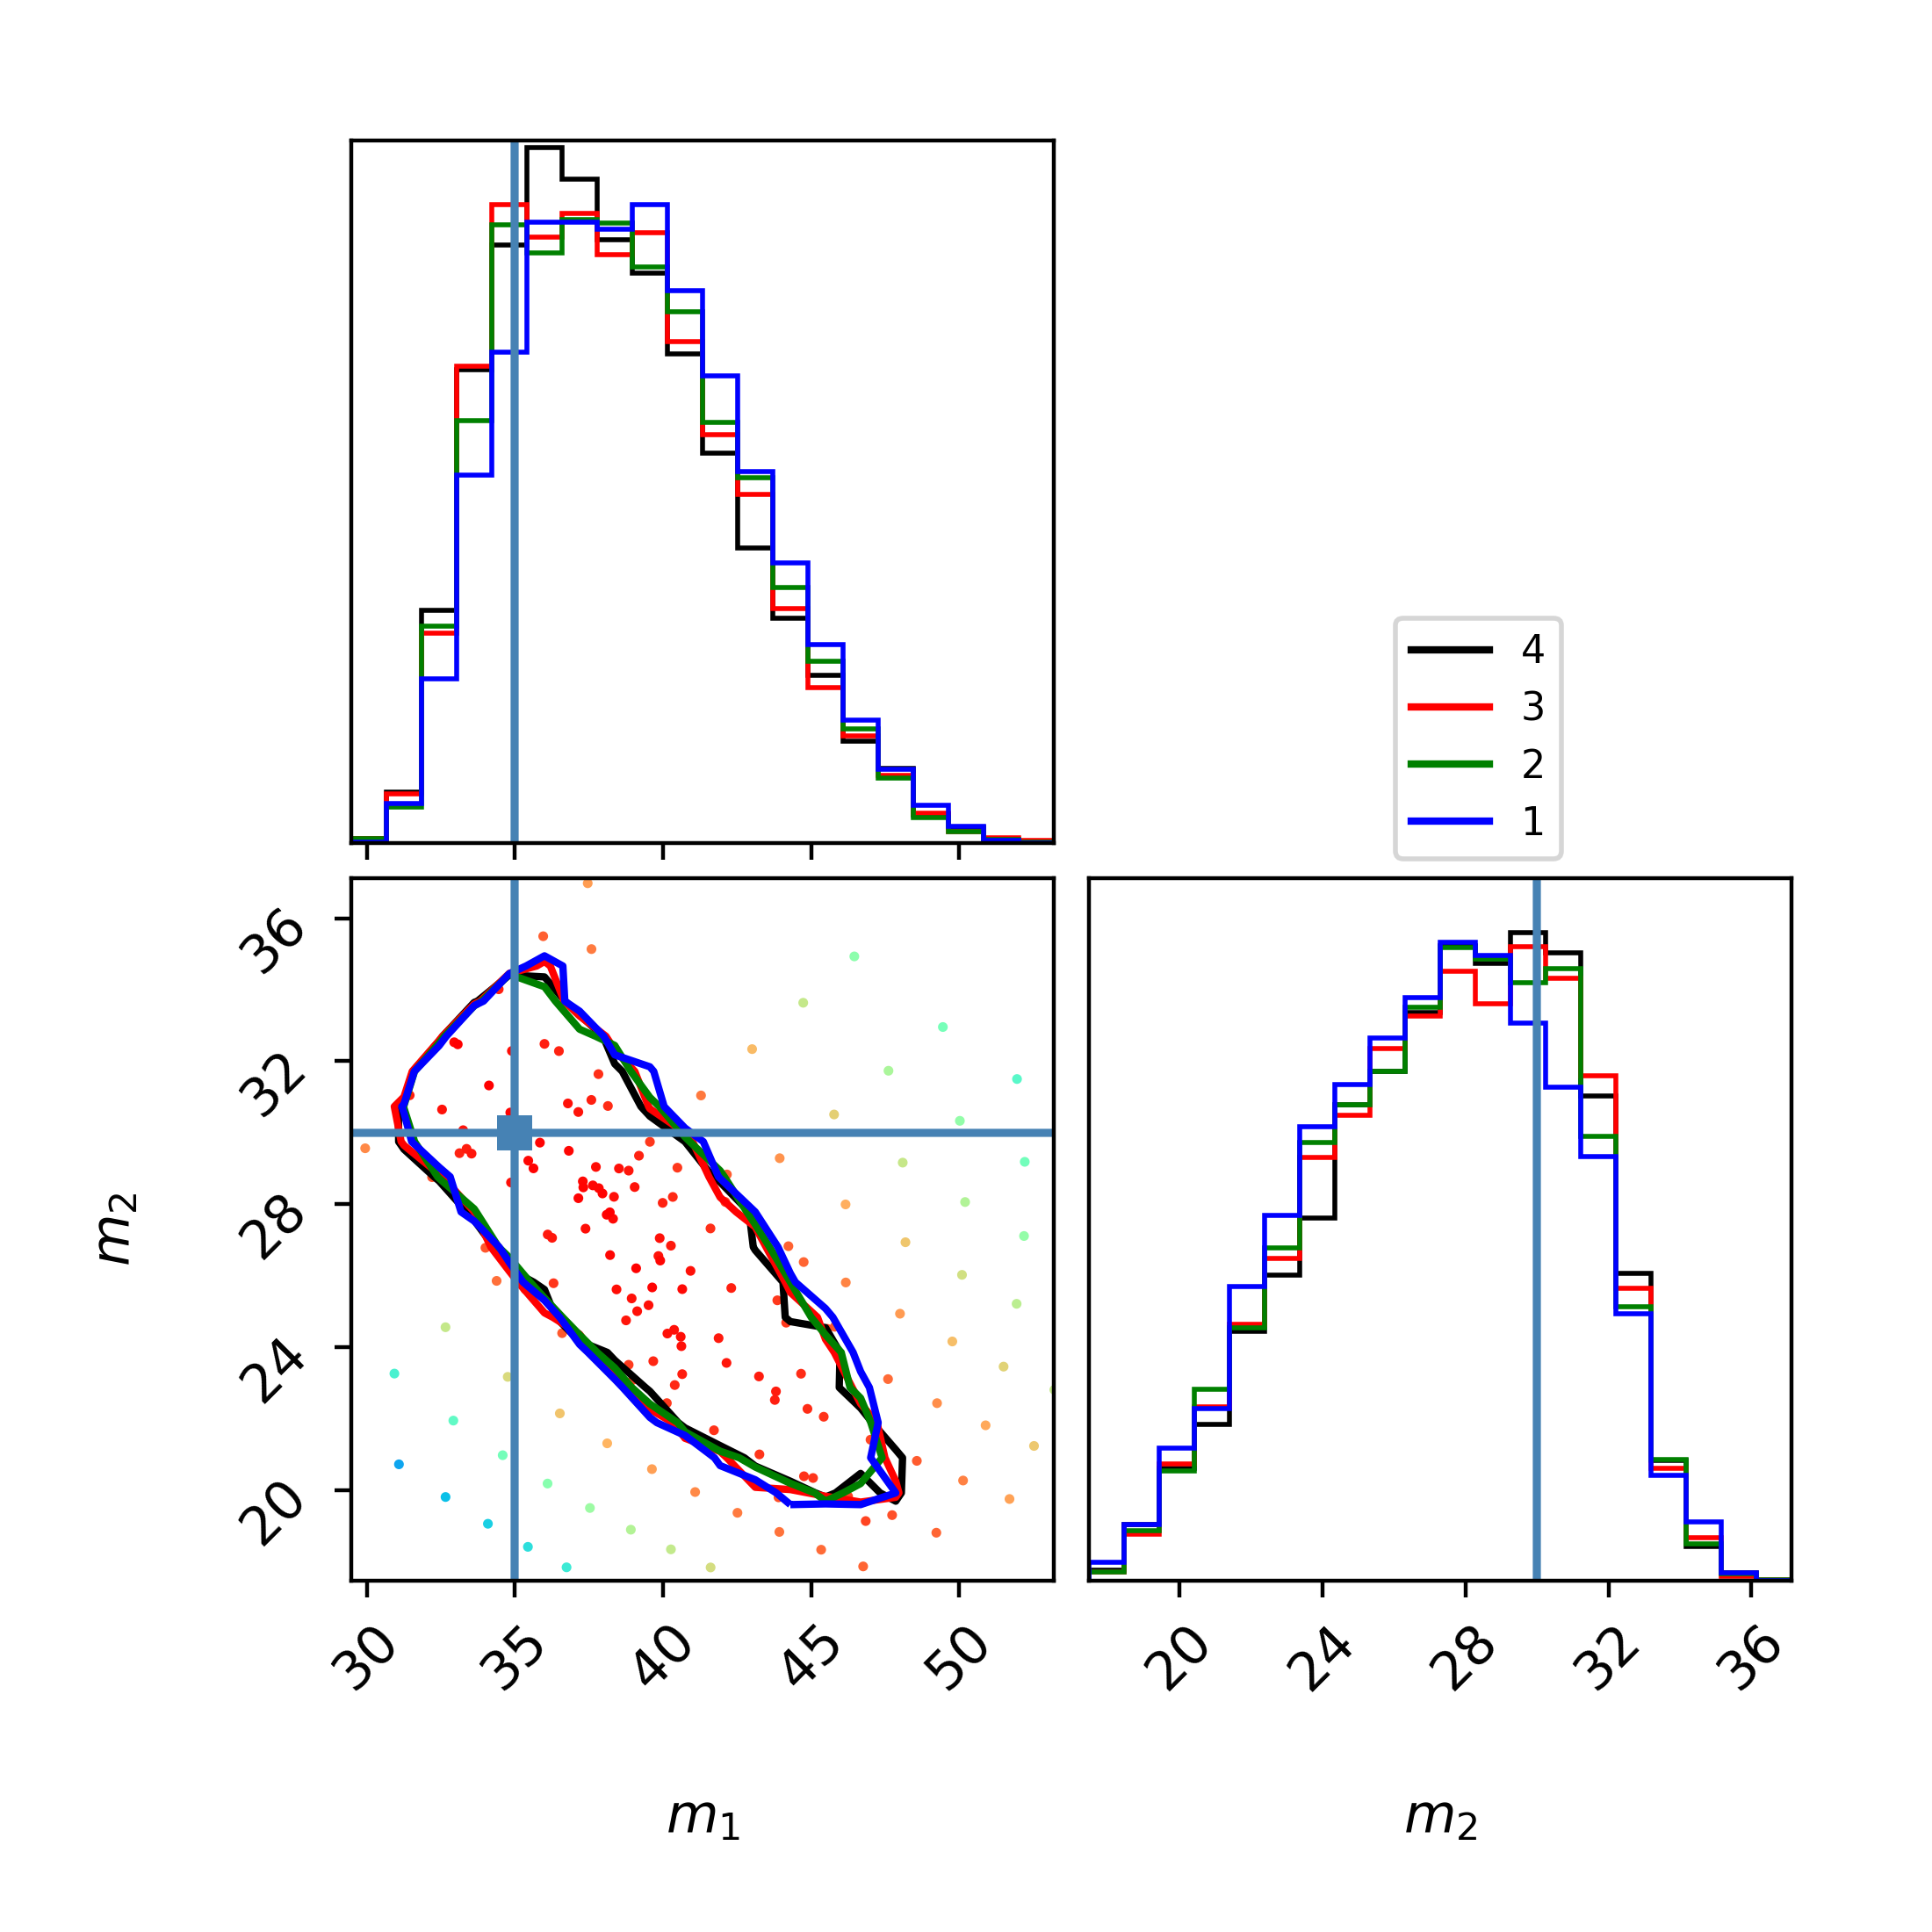
\includegraphics[width=0.45\textwidth]{figures/bbh_zerospin_m1_m2.png}
% 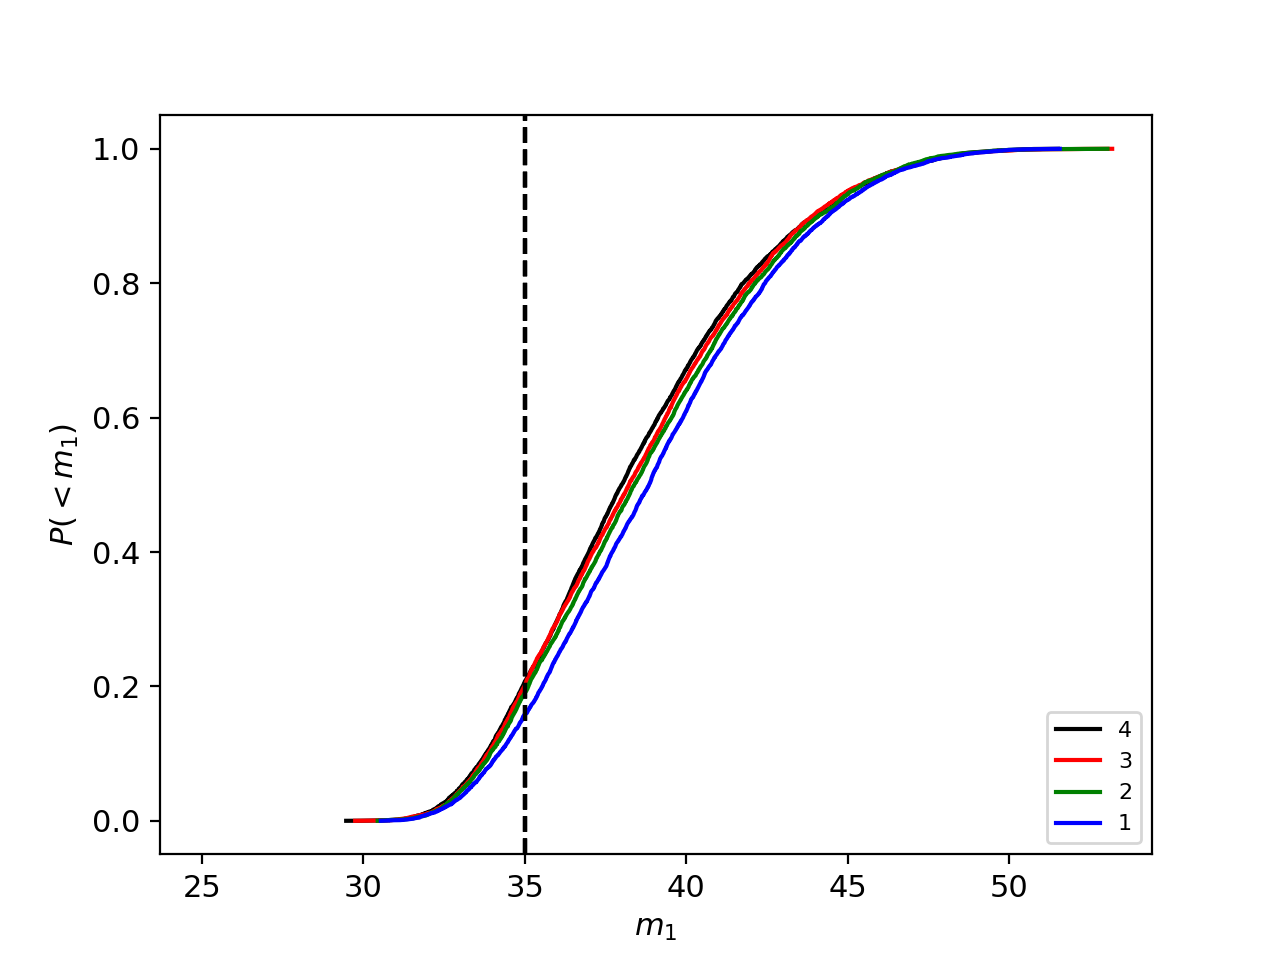
\includegraphics[width=0.45\textwidth]{figures/bbh_zerospin_m1_cum.png}
% % python plot_mean_variance.py --convergence-file 20190203-bbh-zerospin-batch_gpu_lowlatency_meanVar.dat  --output bbh_zerospin_lnL_meanVar
% 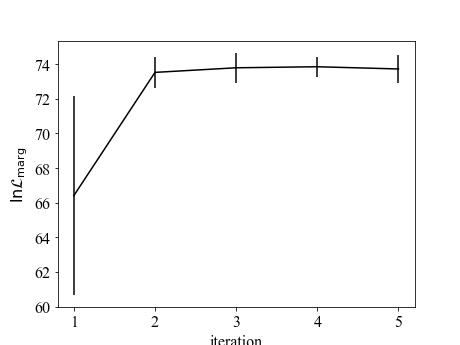
\includegraphics[width=0.45\textwidth]{figures/bbh_zerospin_lnL_meanVar.png}
% % python plot_convergence.py --convergence-file 20190203-bbh-zerospin-batch_gpu_lowlatency.dat
% 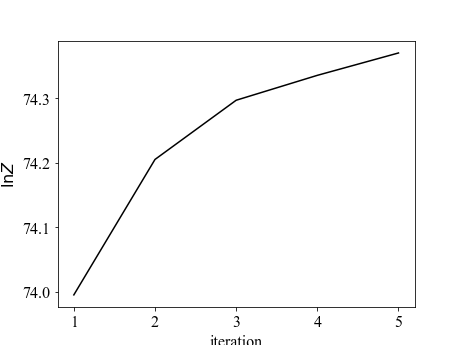
\includegraphics[width=0.45\textwidth]{figures/bbh_zerospin_lnL_converge.png}
% \caption{\label{fig:BBH:MultiIterate}\textbf{Convergence of BBH analysis: Zero spin}: Results for marginal posterior distributions
%   of our fiducial synthetic binary black hole.  Solid contours show credible intervals; solid one-dimensional distributions
%   show marginal CDFs and PDFs for the corresponding variable; and colored points indicate the location $\bm{\lambda}$ and
%   value of the underlying marginalized likelihood evaluations.   
% %The corresponding dotted curves show an analysis using   only the $m=\pm 2$ modes \editremark{perform both} 
% \emph{Left panel } Posterior distribution
%   over  $\mc$ and
%   $\delta=(m_1-m_2)/M$.    \emph{Right panel}: Marginal 1d CDFs of $\mc$, showing convergence.
% \emph{Bottom left}: Mean and variance of  \AddedResponse{the array $\ln{\cal L}_{\rm marg}(\bm{\lambda}_j)$  for
% $j=1,2,\ldots N_{\rm eval}$ indexing all candidate sets of intrinsic parameters $\bm{\lambda}_j$ performed in that iteration},  showing that after the
% first iteration the
% candidate points are consistent with the posterior (i.e., no proposed point has very low $\ln {\cal L}_{\rm marg}$).
% \emph{Bottom right panel}: The estimated evidence $Z = \int d\bm{\lambda} {\cal L}_{\rm marg}$ versus iteration number.  As systematic fitting error dominates our
% error budget, Monte Carlo error is not shown.
% }
% \end{figure*}














\section{Conclusions}
\label{sec:conclude}
In Progress, 




* summarize your calculations

* summarize key takeaways

** we WILL find this, measuremeent error can't be too large/infinite!

* contrast /compare with other papers 

* some comments on what it all means for the big picture (dynamical evolution tests for example could be done)














\begin{acknowledgements}
We thank our anonymous referee for the helpful feedback.

\end{acknowledgements}


\appendix
In Progress,




%\bibstyle{unsrt}
\bibliography{paperexport,LIGO-publications}
\end{document}
